% Created with jtex v.1.0.18
\documentclass{article}
\PassOptionsToPackage{short, nodayofweek}{datetime}


% Start Curvenote Definitions

% Pass Options Section
% base
\PassOptionsToPackage{normalem}{ulem}
\PassOptionsToPackage{utf8}{inputenc}

% template
\PassOptionsToPackage{framemethod=TikZ}{mdframed}
\PassOptionsToPackage{x11names, svgnames}{xcolor}

%%% PACKAGES

% base
\usepackage{inputenc}
\usepackage{url}
\usepackage{graphicx}
\usepackage{adjustbox}
\usepackage{amssymb}
\usepackage{amsfonts}
\usepackage{amsmath}
\usepackage{enumitem}
\usepackage{nicefrac}
\usepackage{booktabs}
\usepackage{microtype}
\usepackage{hyperref}
\usepackage{ulem}
\usepackage{enumitem}
\usepackage{float}
\usepackage{datetime}
\usepackage{xkeyval}
\usepackage{framed}
\usepackage{doi}

% template
\usepackage{natbib}
\usepackage{fancyvrb}
\usepackage{mdframed}
\usepackage{xcolor}

%%%


%%%% Setup Section

% base
\graphicspath{{.}}
% template
\sloppy
\newenvironment{aside}{\begin{framed}}{\end{framed}}
\newmdenv[linewidth=2pt,linecolor=CornflowerBlue,topline=false,bottomline=false,rightline=false,leftline=true,skipabove=20,skipbelow=20,leftmargin=20,rightmargin=20]{callout}
\newfloat{code}{thp}{loc}
\floatname{code}{Program}
\raggedbottom
\bibliographystyle{abbrvnat}
\setcitestyle{authoryear,open={(},close={)},semicolon,aysep={,}}

% End Curvenote Definitions




% colors for hyperlinks
\hypersetup{colorlinks=true, allcolors=blue}
\hypersetup{
pdftitle={\@title},
pdfsubject={},
pdfauthor={\@author},
pdfkeywords={},
addtopdfcreator={Written in Curvenote}
}

\usepackage{curvenote}

\title{Novocraft SV Genotyping Report}

\newdate{articleDate}{30}{9}{2024}
\date{\displaydate{articleDate}}

\author{}

\begin{document}

\maketitle

\subsection{Background}

\begin{itemize}
\item Investigating the feasibility of an \textbf{alignment-based SV genotyper}.
\item The functionality is based on Novocraft's HLA algorithm.
\item A list of known structural variants is used to construct alternate contigs.
\item A new reference consisting of the \textbf{reference genome + SV alt contigs} is used for alignment.
\item If an SV from the list is present, more reads from this region are expected to align to the corresponding SV alt contig with a better mapping quality compared to the corresponding reference location.
\item Thus, \textbf{MAPQ} along with other information may be used to select the combination of alleles which best account for the observed reads.
\end{itemize}

\subsection{Assumptions}

\begin{itemize}
\item Let $R_{\text{MAPQ}} = \frac{\text{MAPQ}_{\text{alt}}}{\text{MAPQ}_{\text{ref}}}$.
\item If the sample is \textbf{homozygous alternate}, we expect $\text{MAPQ}_\text{alt} \gg \text{MAPQ}_{\text{ref}}$, and therefore the MAPQ ratio should be very large ($R_{\text{MAPQ}} \gg 1$).
\item If the sample is \textbf{homozygous reference}, we expect $\text{MAPQ}_\text{alt} \ll \text{MAPQ}_{\text{ref}}$, and therefore the MAPQ ratio should be very small ($R_{\text{MAPQ}} \ll 1$).
\item If the sample is \textbf{heterozygous}, we expect $\text{MAPQ}_\text{alt} \approx \text{MAPQ}_{\text{ref}}$ and therefore the MAPQ ratio should be close to 1 ($R_{\text{MAPQ}} \approx 1$).
\end{itemize}

\subsection{Benchmarks to use}

\begin{itemize}
\item HG002 (reads and truth set obtained from \href{https://github.com/human-pangenomics/HG002\_Data\_Freeze\_v1.0}{GIAB})
\item HG005 (reads and truth set obtained from \cite{Duan_2022})
\item HG00513 (reads and truth set obtained from \href{https://www.internationalgenome.org/data-portal/data-collection/hgsvc2}{HGSVC2})
\end{itemize}

\subsection{Observations (in HG002)}

\subsubsection{MAPQ ratio distribution}

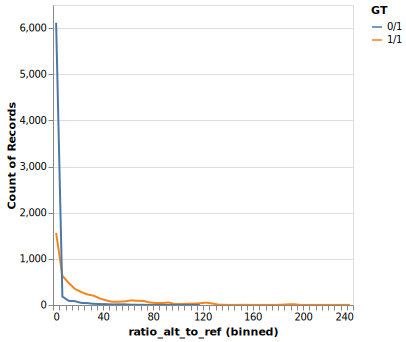
\includegraphics[width=0.7\linewidth]{files/mapq_chart-9fd31293e90b26bea2acdc0f0d71e94c.svg}

\begin{itemize}
\item Transformations (e.g., $\sqrt{R_{\text{MAPQ}}}$ or $\sqrt[3]{R_{\text{MAPQ}}}$) can make the distribution easier to visualize at a glance.
\item How will the distribution of true negatives (homozygous reference) affect genotyping?\begin{itemize}
\item If it does not overlap significantly with the peak, 0/0 should be resolvable and performance characteristics may not be drastically affected.
\end{itemize}
\end{itemize}

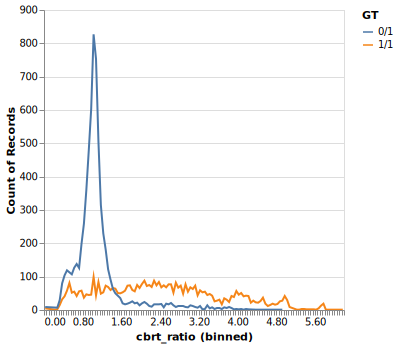
\includegraphics[width=0.7\linewidth]{files/cbrt_mapq_chart-963f8a73154d31ff3df583f26e55e6ee.svg}

\begin{itemize}
\item Zoom in on distirbution of $R_{\text{MAPQ}}$ to select reasonable cutoffs.
\item The $R_{\text{MAPQ}}$ distribution has a mode at around 1, as expected.
\item However, there is some overlap where SVs have an unexpected $R_{\text{MAPQ}}$ for the reported genotype.
\item Using the following cutoff values yields a recall of 78\% (genotype called correctly):
\end{itemize}

\begin{equation}
\text{NaN} = ./. \\
[0,0.2) = 0/0 \\
[0.2,2.8) = 0/1 \\
[2.8,\infty) = 1/1
\end{equation}

\subsection{What does Novotyper do?}

\begin{verbatim}
from novotyper import genotyper as gt

vcf_info = gt.extract_info_from_vcf(sv_vcf, sample)
mapq_bedgraph = gt.read_mapq_bedgraph(mapq_bedgraph)

test_locs = (
    alts_fasta
    |> gt.read_alts_fasta_descriptions
    |> lift(,)(gt.extract_ref_locs_of_alts, gt.extract_sv_locs)
    |*> gt.join_ref_and_sv_locs
    |> gt.define_alt_test_locs
    |> gt.add_vcf_info_to_test_locs$(?, vcf_info)
    |> gt.get_pass_variants
)

ratio_results = (
    test_locs
    |> lift(,)(gt.get_ref_test_locs, gt.get_alt_test_locs)
    |> map$(gt.calculate_mapq$(?, mapq_bedgraph))
    |*> gt.join_and_calculate_mapq_ratio$(test_locs)
    |> gt.predict_genotype$(?, 0.2, 2.8)
)
\end{verbatim}

\begin{itemize}
\item These functions are defined below (Novotyper~code).
\end{itemize}

\subsection{HG002 genotype prediction results}

\bigskip\noindent
\begin{tabular}{p{\dimexpr \linewidth-2\tabcolsep}}
\toprule
RECALL \\
\hline
78.08552373479796 \\
\bottomrule
\end{tabular}

\bigskip\bigskip\noindent
\begin{tabular}{p{\dimexpr 0.200\linewidth-2\tabcolsep}p{\dimexpr 0.200\linewidth-2\tabcolsep}p{\dimexpr 0.200\linewidth-2\tabcolsep}p{\dimexpr 0.200\linewidth-2\tabcolsep}p{\dimexpr 0.200\linewidth-2\tabcolsep}}
\toprule
GT\_unphased & ./. & 0/0 & 0/1 & 1/1 \\
\hline
0/1 & 0.00201787 & 0.0762468 & 0.774142 & 0.147593 \\
1/1 & 0.00258309 & 0.0466678 & 0.161874 & 0.788875 \\
\bottomrule
\end{tabular}

\bigskip\bigskip\noindent
\begin{tabular}{p{\dimexpr 0.250\linewidth-2\tabcolsep}p{\dimexpr 0.250\linewidth-2\tabcolsep}p{\dimexpr 0.250\linewidth-2\tabcolsep}p{\dimexpr 0.250\linewidth-2\tabcolsep}}
\toprule
SVTYPE & Matching genotypes & Total & \% Correct \\
\hline
DEL & 4352 & 5464 & 79.6486 \\
INS & 5600 & 7281 & 76.9125 \\
\bottomrule
\end{tabular}

\bigskip\subsection{Things to consider for further development}

\subsubsection{Overlaps in $R_{\text{MAPQ}}$ distributions}

\begin{itemize}
\item Ideally the distributions for 0/0, 0/1, and 1/1 should be separable to distinguish genotypes.
\item Overlaps mean \textbf{some incorrectly called genotypes may be inevitable}.\begin{itemize}
\item Also, MAPQ involves probability.
\end{itemize}


\item Is there a systematic cause that can be addressed?\begin{itemize}
\item MAPQ ratio close to 1 (implying 0/1) but actually 1/1.
\item MAPQ ratio very low (implying 0/0) but actually 0/1 or 1/1.
\item MAPQ ratio very high (implying 1/1) but actually 0/0 or 0/1.
\end{itemize}


\item Most of them tend to be in what look like repetitive or low-complexity regions.
\item Is there a reason for the ``spikes'' in the MAPQ distributions near 0?
\end{itemize}

\subsubsection{Generalizability of cutoffs}

\begin{itemize}
\item Can the cutoffs be applied to other samples?\begin{itemize}
\item The distributions could be affected by things such as sequencing parameters (coverage, etc.).
\end{itemize}


\item To investigate cutoffs, other benchmarks (e.g. HGSVC2) can be used to see if the distributions are similar, or to combine all samples and see the overall distribution.\begin{itemize}
\item I tried to run it with the HG005 and HG00513 benchmarks, but \texttt{novoSV} and \texttt{novoindex} raise errors with the truth set VCFs.
\end{itemize}
\end{itemize}

\subsubsection{Precision}

\begin{itemize}
\item To assess precision, we need to include \textbf{true negative SVs} (homozygous reference).\begin{itemize}
\item Use the HGSVC2 benchmark VCF, which contains 0/0 variants.
\item Use simulated reads, so you are completely certain about the alleles.
\item Use the calls from an SV caller and see whether precision can be improved without negatively affecting recall.
\end{itemize}


\item A variant may be detected by some methods but \textbf{filtered out} due to not meeting certain criteria.\begin{itemize}
\item There are some examples of this in the GIAB small variant benchmarks.
\item This complicates the process of finding true negatives with which to assess precision.
\end{itemize}
\end{itemize}

\subsubsection{Other considerations}

\begin{itemize}
\item \textbf{Split multiallelic VCF files} prior to alt contig generation (so that the only possible genotypes are 0/0, 0/1, 1/1, or ./.).
\item Should there be a \textbf{minimum MAPQ}?
\item Should repeat and \textbf{low-complexity regions} be masked?
\item How will it perform on \textbf{other SV types}?\begin{itemize}
\item Duplications and inversions can be treated as insertions.
\item Translocations?
\item Since they are not present or clearly labelled in most benchmarks, how can performance on these SV types be evaluated?
\end{itemize}
\end{itemize}

%

\subsection{Comparison to other genotypers}

\begin{itemize}
\item The novoSV method has some similarities to graph-based SV genotypers (e.g., NPSV, SV2, Paragraph, vg, SVTyper, SVJedi-graph, GraphTyper, BayesTyper)\begin{itemize}
\item These use nodes of a graph to represent the different haplotypes instead of alt contigs.
\item They are usually much faster.
\item Some also struggle with nearby and overlapping SVs.
\end{itemize}


\item The novoSV method can take inspiration from some of their ideas:\begin{itemize}
\item How can other information be incorporated to improve the performance? Can we into consideration the uniqueness of read mapping and alignment counts?
\item NovoAlign takes too long as it has to align to the whole genome. Can alignment be limited to only targeted regions?
\end{itemize}


\item What would be the advantages of novoSV?\begin{itemize}
\item Can it be used to improve the precision of other SV callers by a significant amount?
\end{itemize}
\end{itemize}

\subsection{Known limitations}

\begin{itemize}
\item This method is limited to trying to detect and genotype known SVs.\begin{itemize}
\item It cannot detect \textit{de novo} SVs.
\item A library of known SVs of interest (e.g., those associated with a phenotype or disease, or those previously called by another SV caller) will be useful for this method.
\end{itemize}
\end{itemize}

\section{Novotyper code}

\begin{verbatim}
import re

import pandas as pd
import pyranges as pr
import polars as pl
import bioframe as bf
import numpy as np
import altair as alt
\end{verbatim}

\begin{verbatim}
alt.data_transformers.enable("vegafusion")
\end{verbatim}

\subsection{Load data}

\begin{verbatim}
def read_alts_fasta_descriptions(alts_fasta: Path) -> pl.DataFrame:
    with open(alts_fasta, "r") as file:
        records = re.findall(r">([\d\w_]+) LN:(\d+) .+ rg:([\d\w: -]+)", file.read())

        fields: dict[str, list] = {
            "alt_contig": [],
            "ref_loc": [],
            "alt_contig_len": [],
        }

        for record in records:
            fields["alt_contig"].append(record[0])
            fields["alt_contig_len"].append(record[1])
            fields["ref_loc"].append(record[2])

        data = pl.DataFrame(fields)

    return data


alts_fasta_desc = read_alts_fasta_descriptions("outputs/HG002/alt_scaffolds.fa")

alts_fasta_desc.head()
\end{verbatim}

\subsubsection{Extract reference regions}

\begin{verbatim}
def extract_ref_locs_of_alts(data: pl.DataFrame) -> pr.PyRanges:
    ref_locs_bf = bf.from_any(data.to_series(1).to_list())
    ref_locs_bf["alt_contig"] = pd.Series(data.to_series(0).to_list())
    ref_locs_of_alts = pr.PyRanges(
        ref_locs_bf.rename(
            columns={"chrom": "Chromosome", "start": "Start", "end": "End"}
        )
    )

    return ref_locs_of_alts


ref_locs = extract_ref_locs_of_alts(alts_fasta_desc)
ref_locs.head()
\end{verbatim}

\subsubsection{Extract SV regions}

\begin{verbatim}
def extract_sv_locs(data: pl.DataFrame) -> pr.PyRanges:
    sv_locs = pr.PyRanges(
        data.select("alt_contig", "alt_contig_len")
        .with_columns(
            pl.col("alt_contig")
            .str.extract_groups(r"(\d+|\w+)_(\d+)_(\d+)_\d")
            .struct.rename_fields(["Chromosome", "Start", "End"])
            .alias("alt_contig_locs"),
            pl.col("alt_contig_len").str.to_integer(),
        )
        .unnest("alt_contig_locs")
        .with_columns(pl.col(["Start", "End"]).str.to_integer())
        .to_pandas()
    )

    return sv_locs


sv_locs = extract_sv_locs(alts_fasta_desc)
sv_locs.head()
\end{verbatim}

\subsubsection{Join regions}

\begin{verbatim}
def join_ref_and_sv_locs(
    ref_locs_of_alts: pr.PyRanges, sv_locs: pr.PyRanges
) -> pd.DataFrame:
    locs = sv_locs.df.join(ref_locs_of_alts.df, rsuffix="_ref").drop(
        columns=["alt_contig_ref", "Chromosome_ref"]
    )

    return locs


locs = join_ref_and_sv_locs(ref_locs, sv_locs)
locs.head()
\end{verbatim}

\subsubsection{Get subregions over which MAPQ will be tested}

\begin{verbatim}
def define_alt_test_locs(locs: pd.DataFrame) -> pd.DataFrame:
    test_locs = locs.copy()

    # Get size of context to determine where on alt to start testing
    test_locs["Start_alt_test"] = test_locs["Start"] - test_locs["Start_ref"]

    # Determine where to end testing
    test_locs["End_alt_test"] = np.where(
        test_locs["alt_contig_len"] == 1801,
        test_locs["Start"] + 1 - test_locs["Start_ref"],
        test_locs["Start_alt_test"] + test_locs["alt_contig_len"] - 1801,
    )

    return test_locs


test_locs = define_alt_test_locs(locs)
test_locs.head()
\end{verbatim}

\subsubsection{Read in VCF to filter for only PASS variants}

\begin{verbatim}
def extract_info_from_vcf(vcf_file: Path, sample: str) -> pd.DataFrame:
    vcf = (
        pl.read_csv(
            vcf_file,
            separator="\t",
            comment_prefix="#",
            has_header=False,
            new_columns=[
                "CHROM",
                "POS",
                "ID",
                "REF",
                "ALT",
                "QUAL",
                "FILTER",
                "INFO",
                "FORMAT",
                sample,
            ],
            schema_overrides={"CHROM": pl.String},
        )
        .with_columns(
            pl.col("INFO")
            .str.extract_groups(r"SVLEN=([ -\d]+);")
            .cast(pl.Int32)
            .alias("SVLEN")
            .struct.rename_fields(["SVLEN"]),
            pl.col("INFO")
            .str.extract_groups(r"SVTYPE=(\w+);")
            .alias("SVTYPE")
            .struct.rename_fields(["SVTYPE"]),
            pl.col(sample).str.extract(r"^([\d.\/\|]*):").alias("GT"),
        )
        .unnest(["SVLEN", "SVTYPE"])
        .select(["FILTER", "GT", "SVLEN", "SVTYPE"])
        .to_pandas()
    )

    return vcf


vcf_info = extract_info_from_vcf("resources/HG002/HG002_SVs_Tier1_v0.6.ALL.vcf", "HG002")
vcf_info.head()
\end{verbatim}

\begin{verbatim}
def add_vcf_info_to_test_locs(locs: pd.DataFrame, vcf: pd.DataFrame) -> pd.DataFrame:
    locs_with_info = pd.concat([locs, vcf], axis=1)
    locs_with_info.insert(1, "alt_start", [0] * locs_with_info.shape[0])
    return locs_with_info


test_locs_with_info = add_vcf_info_to_test_locs(test_locs, vcf_info)
test_locs_with_info.head()
\end{verbatim}

\begin{verbatim}
def get_pass_variants(locs: pd.DataFrame) -> pd.DataFrame:
    return locs.query('FILTER == "PASS" or FILTER == "."')


test_locs_with_info_pass_only = get_pass_variants(test_locs_with_info)
test_locs_with_info_pass_only
\end{verbatim}

\subsubsection{Separate ref and alt test locs}

\begin{verbatim}
def get_ref_test_locs(test_locs: pd.DataFrame) -> pd.DataFrame:
    return test_locs.copy()[["alt_contig", "Chromosome", "Start", "End"]]


ref_test_locs = get_ref_test_locs(test_locs_with_info_pass_only)
ref_test_locs
\end{verbatim}

\begin{verbatim}
def get_alt_test_locs(test_locs: pd.DataFrame) -> pd.DataFrame:
    alt_test_locs = test_locs.copy()
    alt_test_locs["Chromosome"] = alt_test_locs["alt_contig"]
    alt_test_locs = alt_test_locs.copy()[
        ["alt_contig", "Chromosome", "Start_alt_test", "End_alt_test"]
    ].rename(columns={"Start_alt_test": "Start", "End_alt_test": "End"})

    return alt_test_locs


alt_test_locs = get_alt_test_locs(test_locs_with_info_pass_only)
alt_test_locs
\end{verbatim}

\subsection{Prepare MAPQ}

\begin{verbatim}
def read_mapq_bedgraph(bedgraph_file: Path) -> pr.PyRanges:
    bedgraph: pd.DataFrame = pd.read_csv(
        bedgraph_file,
        sep=" ",
        header=0,
        skiprows=1,
        names=["Chromosome", "Start", "End", "MAPQ"],
        dtype={"Chromosome": str},
    )

    return pr.PyRanges(bedgraph)


mapq_bedgraph = read_mapq_bedgraph("outputs/HG002/sv.sorted.bedgraph")
mapq_bedgraph
\end{verbatim}

\subsubsection{Calculate MAPQ over REF test locs}

\begin{verbatim}
def calculate_mapq(test_locs: pd.DataFrame, mapq_bedgraph: pd.DataFrame):
    return (
        pr.PyRanges(test_locs)
        .extend(100)
        .join(mapq_bedgraph)
        .df.groupby("alt_contig")
        .agg({"MAPQ": "mean"})
    )


ref_mapq = calculate_mapq(ref_test_locs, mapq_bedgraph)
ref_mapq
\end{verbatim}

\subsubsection{Calculate MAPQ over ALT test locs}

\begin{verbatim}
alt_mapq = calculate_mapq(alt_test_locs, mapq_bedgraph)
alt_mapq
\end{verbatim}

\subsection{Join all results and calculate $R_{\text{MAPQ}}$}

\begin{verbatim}
def join_and_calculate_mapq_ratio(
    locs_with_info: pd.DataFrame, ref_mapq: pd.DataFrame, alt_mapq: pd.DataFrame
):
    results = (
        locs_with_info.set_index("alt_contig")
        .join(ref_mapq, rsuffix="_ref")
        .join(alt_mapq, rsuffix="_alt")
        .reset_index()
        .set_index(["Chromosome", "Start", "End"])
    )

    results["ratio_alt_to_ref"] = results["MAPQ_alt"] / results["MAPQ"]

    results["sqrt_ratio"] = np.sqrt(results["ratio_alt_to_ref"])
    results["cbrt_ratio"] = np.cbrt(results["ratio_alt_to_ref"])

    return results


results = join_and_calculate_mapq_ratio(
    test_locs_with_info_pass_only,
    ref_mapq,
    alt_mapq
)
results
\end{verbatim}

\subsection{Plot distributions of MAPQ ratio}

\begin{verbatim}
def plot_mapq_distribution(results: pd.DataFrame) -> tuple[alt.Chart]:
    inf = np.inf

    mapq_chart = (
        alt.Chart(
            results.query("not ratio_alt_to_ref.isna() and ratio_alt_to_ref != @inf")
        )
        .mark_line()
        .encode(
            alt.X("ratio_alt_to_ref:Q").bin(maxbins=100),
            y="count()",
            color=alt.Color("GT"),
        )
        .interactive()
    )

    mapq_chart_detailed = (
        alt.Chart(
            results.query("not ratio_alt_to_ref.isna() and ratio_alt_to_ref != @inf")
        )
        .mark_line()
        .encode(
            alt.X("ratio_alt_to_ref:Q").bin(maxbins=5000),
            y="count()",
            color=alt.Color("GT"),
        )
        .interactive()
    )

    sqrt_mapq_chart = (
        alt.Chart(
            results.query("not ratio_alt_to_ref.isna() and ratio_alt_to_ref != @inf")
        )
        .mark_line()
        .encode(
            alt.X("sqrt_ratio:Q").bin(maxbins=250), y="count()", color=alt.Color("GT")
        )
        .interactive()
    )

    cbrt_mapq_chart = (
        alt.Chart(
            results.query("not ratio_alt_to_ref.isna() and ratio_alt_to_ref != @inf")
        )
        .mark_line()
        .encode(
            alt.X("cbrt_ratio:Q").bin(maxbins=250), y="count()", color=alt.Color("GT")
        )
        .interactive()
    )

    return (mapq_chart, mapq_chart_detailed, sqrt_mapq_chart, cbrt_mapq_chart)


mapq_chart, mapq_chart_detailed, sqrt_mapq_chart, cbrt_mapq_chart = plot_mapq_distribution(results)

out_dir = "outputs/HG002"
mapq_chart.save(f"{out_dir}/mapq_chart.svg")
mapq_chart_detailed.save(f"{out_dir}/mapq_chart_detailed.svg")
sqrt_mapq_chart.save(f"{out_dir}/sqrt_mapq_chart.svg")
cbrt_mapq_chart.save(f"{out_dir}/cbrt_mapq_chart.svg")
\end{verbatim}

\subsection{Make predictions based on $R_{\text{MAPQ}}$}

\begin{equation}
\text{NaN} = ./. \\
[0,0.2) = 0/0 \\
[0.2,2.8) = 0/1 \\
[2.8,\infty) = 1/1 \\
\end{equation}

\begin{verbatim}
def predict_genotype(
    results: pd.DataFrame, lower_het_bound: float, upper_het_bound: float
) -> pd.DataFrame:
    predictions = results.copy()

    predictions["prediction"] = np.where(
        results["ratio_alt_to_ref"].isna(),
        "./.",
        np.where(
            results["ratio_alt_to_ref"] >= upper_het_bound,
            "1/1",
            np.where(results["ratio_alt_to_ref"] < lower_het_bound, "0/0", "0/1"),
        ),
    )

    predictions["GT_unphased"] = np.where(
        predictions["GT"].str.contains('/'),
        predictions["GT"],
        predictions["GT"].map(
        {"0|0": "0/0", "0|1": "0/1", "1|0": "0/1", "1|1": "1/1"}),
    )

    predictions["GT_concordance"] = (
        predictions["prediction"] == predictions["GT_unphased"]
    )

    return predictions


predictions = predict_genotype(results, 0.2, 2.8)
predictions
\end{verbatim}

\begin{verbatim}
def calculate_performance(predictions: pd.DataFrame) -> str:
    recall = 100 * sum(predictions["GT_concordance"]) / predictions.shape[0]

    correct_predictions_by_svtype = predictions.groupby("SVTYPE").agg(
        {"GT_concordance": ["sum", "count"]}
    )
    correct_predictions_by_svtype["pct"] = (
        100
        * correct_predictions_by_svtype[("GT_concordance", "sum")]
        / correct_predictions_by_svtype[("GT_concordance", "count")]
    )

    contingency_table = pd.crosstab(
        predictions["GT_unphased"], predictions["prediction"], normalize="index"
    )

    return "\n\n".join(
        [f"|RECALL|\n| - - -|\n|{recall}|",
        contingency_table.to_markdown(),
        correct_predictions_by_svtype.to_markdown(),]
    )


performance = calculate_performance(predictions)

with open(f"{out_dir}/summary.md", "w") as file:
    print(performance, file=file)
\end{verbatim}

\clearpage
\bibliography{main.bib}

\end{document}
